\chapter{信号処理技術の画像データへの応用}

本章では,離散フーリエ変換の画像データへの応用について紹介する.

\section{離散フーリエ変換の画像データへの応用}

これまでの離散フーリエ変換(式(\ref{eq:dft}))は時間空間の1次元離散データにおける
周波数成分を抽出し,離散逆フーリエ変換(式(\ref{eq:idft}))を用いて
時間領域のデータへ復元していた.
この1次元データ上での離散フーリエ変換を画像データへ応用するには,画像を2次元の
時間空間における離散データ$f(x, y)$とみなし,$x, y$それぞれの方向に対して
離散フーリエ変換(式(\ref{eq:dft_2d}))することで,2次元の周波数成分$F(u, v)$を算出できる.
\begin{align}
  F(u, v) = \sum_{x = 0}^{M-1} \sum_{y = 0}^{N-1} f(x, y) e ^ {- 2 \pi \left(\frac{ux}{M} + \frac{vy}{N} \right) j} \label{eq:dft_2d}
\end{align}
\autoref{fig:input_example},\autoref{fig:dft_example}
に画像データへ離散フーリエ変換を行った例を示す.
\autoref{fig:input_example}は入力画像であり,
\autoref{fig:dft_example}は入力画像の周波数領域である.
この図では,図の中心に近い領域は低周波成分を示し,中心から離れていくほど高周波成分を示している.
\autoref{Fig:dft_example}に対して信号処理にて用いられているバンドパスフィルタを
用いることで信号処理技術でのフィルタ処理を画像データに応用できる.

離散フーリエ逆変換も式(\ref{eq:dft_2d})と同様に$(u, v)$それぞれの方向に対して
逆変換を行うことで\autoref{fig:dft_example}から元の画像へ復元できる(式(\ref{eq:idft_2d})).
\begin{align}
  f(x, y) = \frac{1}{MN} \sum_{u = 0}^{M-1} \sum_{v = 0}^{N-1} F(u, v) e ^ {2 \pi \left(\frac{ux}{M} + \frac{vy}{N} \right) j} \label{eq:idft_2d}
\end{align}
\iffigure
\begin{figure}[h]
  \centering
  \begin{minipage}{.45\hsize}
    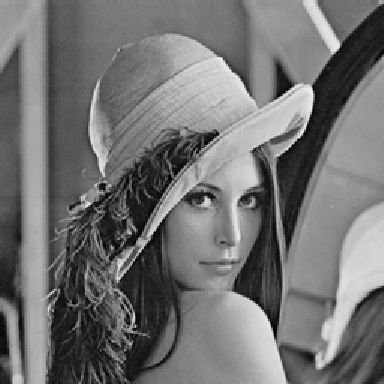
\includegraphics[clip, width=\textwidth]{figure/Lenna.pdf}
    \caption{入力画像}
    \label{fig:input_example}
  \end{minipage}
  \begin{minipage}{.45\hsize}
    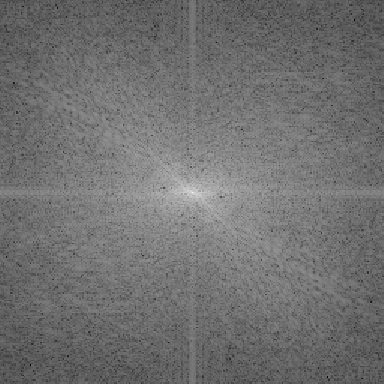
\includegraphics[clip, width=\textwidth]{figure/Lenna_dft.pdf}
    \caption{入力画像の周波数成分}
    \label{fig:dft_example}
  \end{minipage}
\end{figure}
\fi
